\section{\uppercase{Progressive strategy for calibrating a binary BCI}}
\label{sec:calibration_eval}

\noindent In the previous section, we found that our compression technique can speed up an SVM classifier without significant detriment to BCI accuracy. However, it must also allow users to quickly calibrate the system to their personal physiological signals.

In this section, we evaluate a strategy for user calibration in which mental gestures are recorded progressively on an ``as needed'' basis. Using  quantized signals with a resolution of 100 bins, we measure user calibration time (the time it takes a user to achieve a threshold accuracy with the BCI) and the classification accuracy each user achieves after calibration. 

Our calibration strategy takes sixty-second sample recordings of mental gestures and splices them into 120 $\sfrac{1}{2}$-second chunks. By performing seven-fold cross-validation on sample data from a pair of mental gestures, we make an estimate of how easily discriminable these gestures are by our classifier. With this technique, we only need to identify the most promising (highest-performing) of candidate gesture pairs for further testing

In addition, we seek to minimize the amount of time users spend recording samples of mental gestures. One way to minimize this time is to first test the subset of gestures most likely to yield strong performance. For each subject, we perform an exhaustive search of the 21 best-performing gesture pairs and record the frequency of each gesture's occurrence in a best-case pair (Table \ref{table:name}). Assuming that we can establish a consistent ordering of best-performing mental gestures for a target population, we use this data to inform the order in which our calibration strategy prompts the user to perform gestures.


\begin{table}[!h]
%  \vspace{-0.2cm}
  \centering
  \begin{tabular}{ | l | l | l | p{5cm} |}
  \hline
  Gesture & Frequency \\ \hline
  \textit{color} & 10 \\ \hline
  \textit{breathing} & 5 \\ \hline
  \textit{pass} & 4 \\ \hline
  \textit{sport} & 3 \\ \hline
  \textit{finger} & 2 \\ \hline
  \textit{song} & 2 \\ \hline
  \textit{audio} & 2 \\ \hline
  \end{tabular}
  \caption{Frequency of each mental gestures's occurrence in a pair that achieves highest classification accuracy for a subject.}
  \label{table:name}
%  \vspace{-0.1cm}
\end{table}

The progressive strategy starts with three gestures most commonly associated with best-case performance (\textit{color}, \textit{breathing}, \textit{pass}) for an initial user calibration time of 180 seconds (60 seconds per gesture). We then cross-validate every permutation of two of these gestures (i.e., \textit{color} versus \textit{breathing}, \textit{color} versus \textit{pass}, \textit{breathing} versus \textit{pass}). The gesture pair with the highest mean score across cross-validation rounds is selected for an additional testing session, in which the remaining 80 seconds of recordings for both gestures are used to generate an estimate of the classifier's accuracy on new EEG signals.

If the score on this additional testing procedure is below 75\%, a commonly used threshold for BCI literacy \cite{vidaurre_towards_2010}, the user will be prompted to record sixty seconds of the next candidate mental gesture (e.g. \textit{sport}). We repeat the above process on unexplored pairs until a pair achieves over 75\% accuracy on post-calibration data, or until all combinations have been evaluated.

\begin{figure}[!h]
  \vspace{-0.2cm}
  \centering

  % Define block styles
  \tikzstyle{decision} = [diamond, draw, fill=blue!20, 
      text width=6em, text badly centered, node distance=3cm, inner sep=0pt]
  \tikzstyle{block} = [rectangle, draw, fill=yellow!20, 
      text width=6em, text centered, rounded corners, minimum height=4em]
  \tikzstyle{line} = [draw, -latex']
  
  \begin{tikzpicture}[node distance = 2cm, auto, scale=0.8, every node/.style={scale=0.8}]
    \selectcolormodel{gray}
    % Place nodes
    \node [block] (init) {Start};
    \node [block, below of=init, node distance=2.5cm] (firstgestures) {Record samples for first 3 gestures (3 x 60 sec)};
    \node [block, below of=firstgestures, node distance=2cm] (cv) {Cross-validate gesture pairs};
    \node [block, below of=cv, node distance=2cm] (test) {Test best pair (2 x 40 sec)};
    \node [decision, below of=test] (decide) {Best pair $\geq$ 75\% accuracy?};
    \node [block, below of=decide, node distance=3.5cm] (done) {Done};
    \node [block, right of=cv, node distance=4cm] (next) {Record sample of next mental gesture (1 x 60 sec)};
    % Draw edges
    \path [line] (init) -- (firstgestures);
    \path [line] (firstgestures) -- (cv);
    \path [line] (cv) -- (test);
    \path [line] (test) -- (decide);
    \path [line] (decide) -| node [near start] {no} (next);
    \path [line] (next) -- (cv);
    \path [line] (decide) -- node {yes}(done);

  \end{tikzpicture}
  \vspace{0.3cm}
  
  \caption{Progressive calibration routine. We begin with 60 second recordings of the three best-performing gestures (Table \ref{table:name}). We then perform seven-fold cross-validation on each pair of gestures. The pair that scored highest on cross-validation is selected for testing on an additional 80 seconds of data, 40 from each gesture. If this test fails to reach 75\% accuracy, we prompt the user to record a 60 second sample of the next highest-scoring gesture and repeat the cross-validation process on all new (unexplored) gesture pairs.}

  \label{fig:calibration_schematic}
  \vspace{-0.1cm}
\end{figure}

%\subsection{Results}

For the given set of seven candidate gestures, the baseline exhaustive search strategy requires 2100 seconds of calibration time (60 seconds times 7 gestures plus 80 seconds times 21 gesture pairs) and produces an average accuracy of 92.5\% across subjects (\textit{$\sigma$} = 0.09). Our progressive strategy takes an average of 374.6 seconds of calibration time (\textit{$\sigma$} = 52.2) and produces an average accuracy of 88.3\% (\textit{$\sigma$} = 0.11).

Figure \ref{fig:calibration_results} shows the results from a subject's perspective. Out of 15 subjects, the progressive calibration strategy allows 66.7\% (10 subjects) to be calibrated in under 5 minutes, and 86.7\% (13 subjects) in under 6 minutes. The remaining two subjects were calibrated in 11 minutes and 22 minutes, respectively. All 15 subjects achieve a minimum of 75\% classification accuracy. Six subjects (40\%) achieve 100\% accuracy.

\begin{figure}[!h]
  \vspace{-0.2cm}
  \centering

  \definecolor{red}{gray}{0.45}
  \definecolor{green}{gray}{0.58}
  \definecolor{blue}{gray}{0.75}
  \definecolor{yellow}{gray}{0.9}
  
  \def\angle{0}
\def\radius{2.9}
\def\cyclelist{{"red","green","blue","yellow"}}
\newcount\cyclecount \cyclecount=-1
\newcount\ind \ind=-1
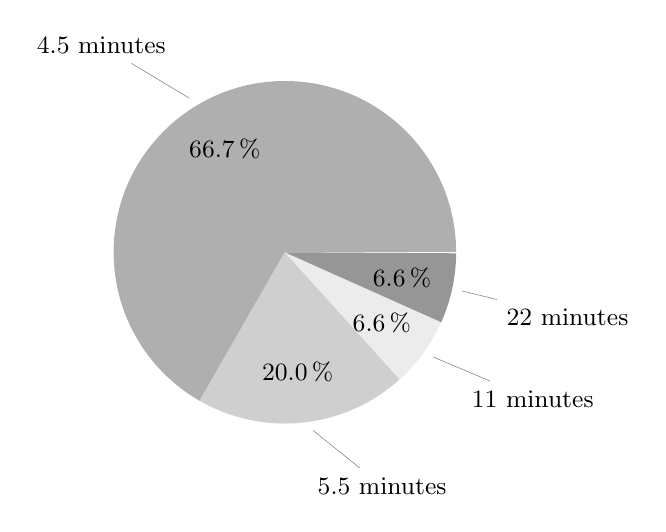
\begin{tikzpicture}[nodes = {font=\small}, scale = .75]
\selectcolormodel{gray}
  \foreach \percent/\name in {
      66.7/4.5 minutes,
      20.0/5.5 minutes,
      6.6/11 minutes,
      6.6/22 minutes
    } {
      \ifx\percent\empty\else               % If \percent is empty, do nothing
        \global\advance\cyclecount by 1     % Advance cyclecount
        \global\advance\ind by 1            % Advance list index
        \ifnum3<\cyclecount                 % If cyclecount is larger than list
          \global\cyclecount=0              %   reset cyclecount and
          \global\ind=0                     %   reset list index
        \fi
        \pgfmathparse{\cyclelist[\the\ind]} % Get color from cycle list
        \edef\color{\pgfmathresult}         %   and store as \color
        % Draw angle and set labels
        \fill[fill={\color!75}] (0,0) -- (\angle:\radius)
          arc (\angle:\angle+\percent*3.6:\radius) -- cycle;
        \node at (\angle+0.5*\percent*3.6:0.7*\radius) {\percent\,\%};
        \node[pin=\angle+0.5*\percent*3.6:\name]
          at (\angle+0.5*\percent*3.6:\radius) {};
        \pgfmathparse{\angle+\percent*3.6}  % Advance angle
        \xdef\angle{\pgfmathresult}         %   and store in \angle
      \fi
    };
  \end{tikzpicture}
  \vspace{0.1cm}
  
  \caption{Calibration time across subjects (top) and classifier accuracy (bottom). The vast majority of subjects achieve acceptable accuracy in under five minutes of training, all but one subject in under 12 minutes, and the remaining subject in 22 minutes. }
  \label{fig:calibration_results}
  \vspace{-0.1cm}
\end{figure}

Our strategy calibrates users to BCI control significantly more quickly than an exhaustive search, and we do not find a significant difference in per-user accuracy between our progressive strategy and an exhaustive search. 

